\documentclass{article}

\usepackage[tmargin=0.5in,bmargin=0.25in]{geometry}
\usepackage{amsmath, amssymb, amsthm}
\usepackage{enumitem}
\usepackage{graphicx}
\graphicspath{{./}}

\title{\vspace{-4ex}Math 341 Homework 7}
\author{Isaac Boaz}

\renewcommand{\arraystretch}{1.2}

\begin{document}

\maketitle

\section*{Problem 3}
\pagebreak
\section*{Problem 8}

\begin{enumerate}[label=\alph*)]
    \item 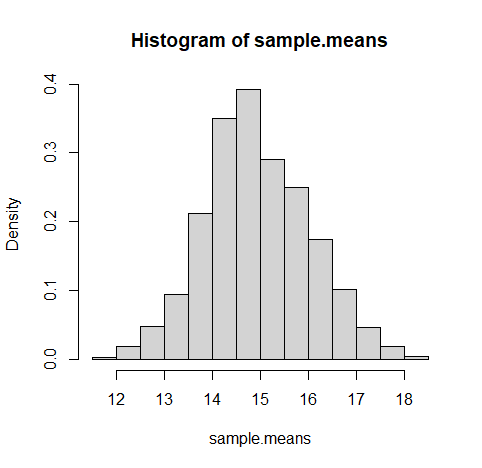
\includegraphics[width=0.5\textwidth]{histogram.png}
    \item Yes, the sample means appear to be normally distributed.
    \item For \(X \sim Exp(15)\), it is know that \(\mu = 15\) and \(\sigma^2 = 225\). By the CLT, this implies that \(\overline{X}\) is approximately normally distributed with mean 15 and variance \(225/n\), where \(n = 200\) in this case. Calculate mean (sample.means) and var (sample.means) and report if these values are close to the theoretical values given by the CLT. \\
          \begin{tabular}{l|rl}
              mean(sample.means) & 14.93516 \\
              var(sample.means)  & 1.162514 \\
              CLTmean(sample.means) & 15 \\
              CLTvar(sample.means) & \(\frac{\sqrt{225}}{\sqrt{200}}\) & \(\approx 1.06066\)  \\
          \end{tabular} \\[1.0em]
          The predicted values given from the CLT are similar to the actual values calculated from the data.
\end{enumerate}

\pagebreak
\section*{Problem 9}
Hogwarts Legacy Pog
\begin{enumerate}[label=\alph*)]
    \item 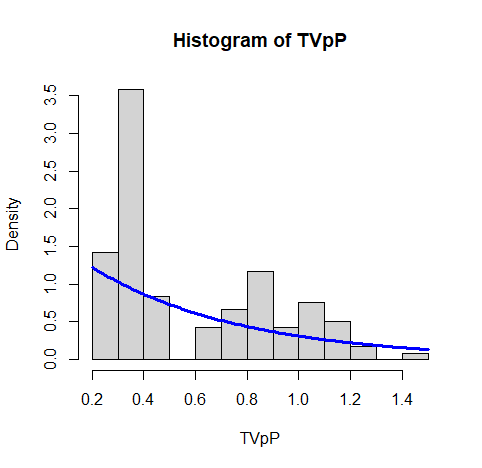
\includegraphics[width=0.5\textwidth]{hogwarts.png} \\
          The exponential distribution assumption does not fit the data very well, though it could be argued that in terms of decay, the PDF does seem to exponentially decay, albeit not very smoothly.
          Given our options from class (exponential, normal, and constant), the best option would indeed be exponential.
    \item Use the CLT.
          \begin{align*}
              P(0.55 \leq & \overline{x}  \leq 0.65) =                                                                                                      \\
                          & = P(\frac{0.55 - \mu}{\sigma/\sqrt{n}} \leq \frac{\overline{x} - \mu}{\sigma/\sqrt{n}} \leq \frac{0.65 - \mu}{\sigma/\sqrt{n}}) \\
          \end{align*}
          \begin{align*}
              n      & = 100 \text{ (`Next 100 TVpP')}  \\
              \mu    & = 0.58 \text{ (Given in R code)} \\
              \sigma & = 0.58                           \\
          \end{align*}
          \begin{align*}
              X \sim Exp(\theta)& ,\ \theta = 0.58                                                                                    \\
              \text{(CLT)} \approx P(\frac{0.55 - 0.58}{0.58/\sqrt{100}} \leq & \mathcal{Z} \leq \frac{0.65 - 0.58}{0.58/\sqrt{100}}) \\
              \approx P(-0.005172414 \leq & \mathcal{Z} \leq 0.01206897)                                                              \\
              & \approx 0.0068782
          \end{align*}
    \item The simulated probability is 0.8351 (compared to the actual probability being \(\approx 0.0068782\)). The difference can be explain by the CLT expecting a normal distribution that can estimate the mean of the whole population. In this case, however, the data is fit to an exponential fit.
\end{enumerate}

\end{document}